\documentclass[12pt,a4paper]{article}
\usepackage[UTF8]{ctex}
\usepackage{amsmath}
\usepackage{graphicx}
\usepackage{booktabs}
\usepackage{geometry}
\usepackage{ulem}
\geometry{left=2.5cm,right=2.5cm,top=2.5cm,bottom=2.5cm}

\title{\Huge{\textbf{\uuline{数\ 据\ 处\ 理}}}}
\author{\uline{少年班学院} \quad 姓名: \uline{李大恕} \quad 学号: \uline{PB24000145} \quad 实验日期: \uline{2025--5--19}}
\date{\today}

\begin{document}
\maketitle

\section{实验题目}
    磁力摆

\section{磁场与电流关系}
    作图表示亥姆霍兹线圈中心磁感应强度与电流强度的关系：

    \begin{figure}[htbp]
        \centering
        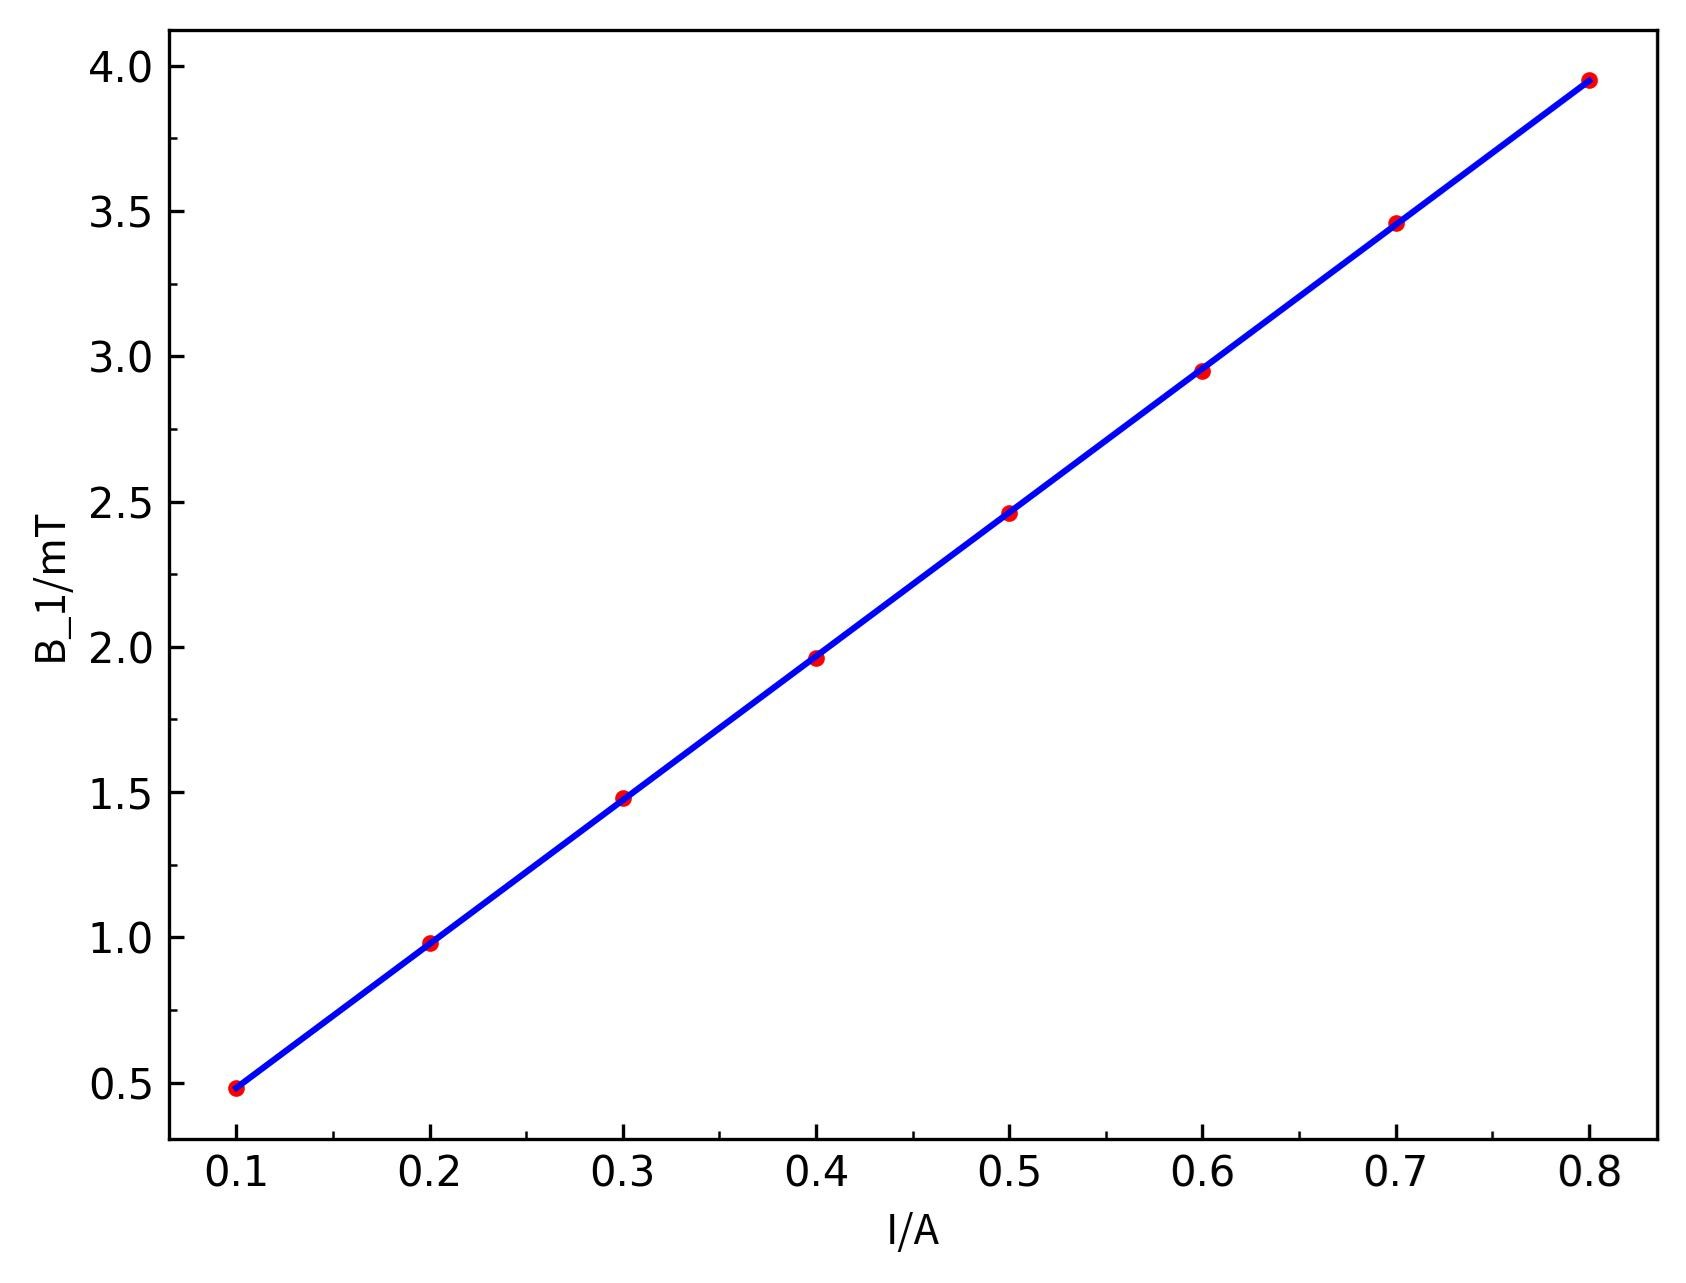
\includegraphics[width=0.8\textwidth]{磁场与电流关系.jpg}
        \caption{\textbf{磁感应强度与电流强度的关系}}
    \end{figure}

    磁感应强度与电流强度的关系为线性关系$B_1=kI$，采用最小二乘法拟合得到：

    斜率
    \[
        k=4.9524\,\mathrm{mT/A}
    \]

\section{不同电流下磁力摆周期}
    由磁力摆周期公式
    \[
        T=2\pi\sqrt{\frac{J}{mB}}
    \]
    其中，$B=B_0+B_1$，$B_0$为地磁场强度，$B_1$为亥姆霍兹线圈中心磁感应强度，$J$为转动惯量，$m$为小磁针磁矩。所以，得$\frac{1}{T^2}=\frac{mB}{4\pi^2J}$，即
    \[
        \frac{1}{T^2}=\frac{m}{4\pi^2J}(B_0+kI)
    \]
    即$\dfrac{1}{T^2}$与$I$成线性关系。设$\dfrac{1}{T^2}=aI+b$，做出图象，并采用最小二乘法拟合得到：
    
    \begin{figure}[htbp]
        \centering
        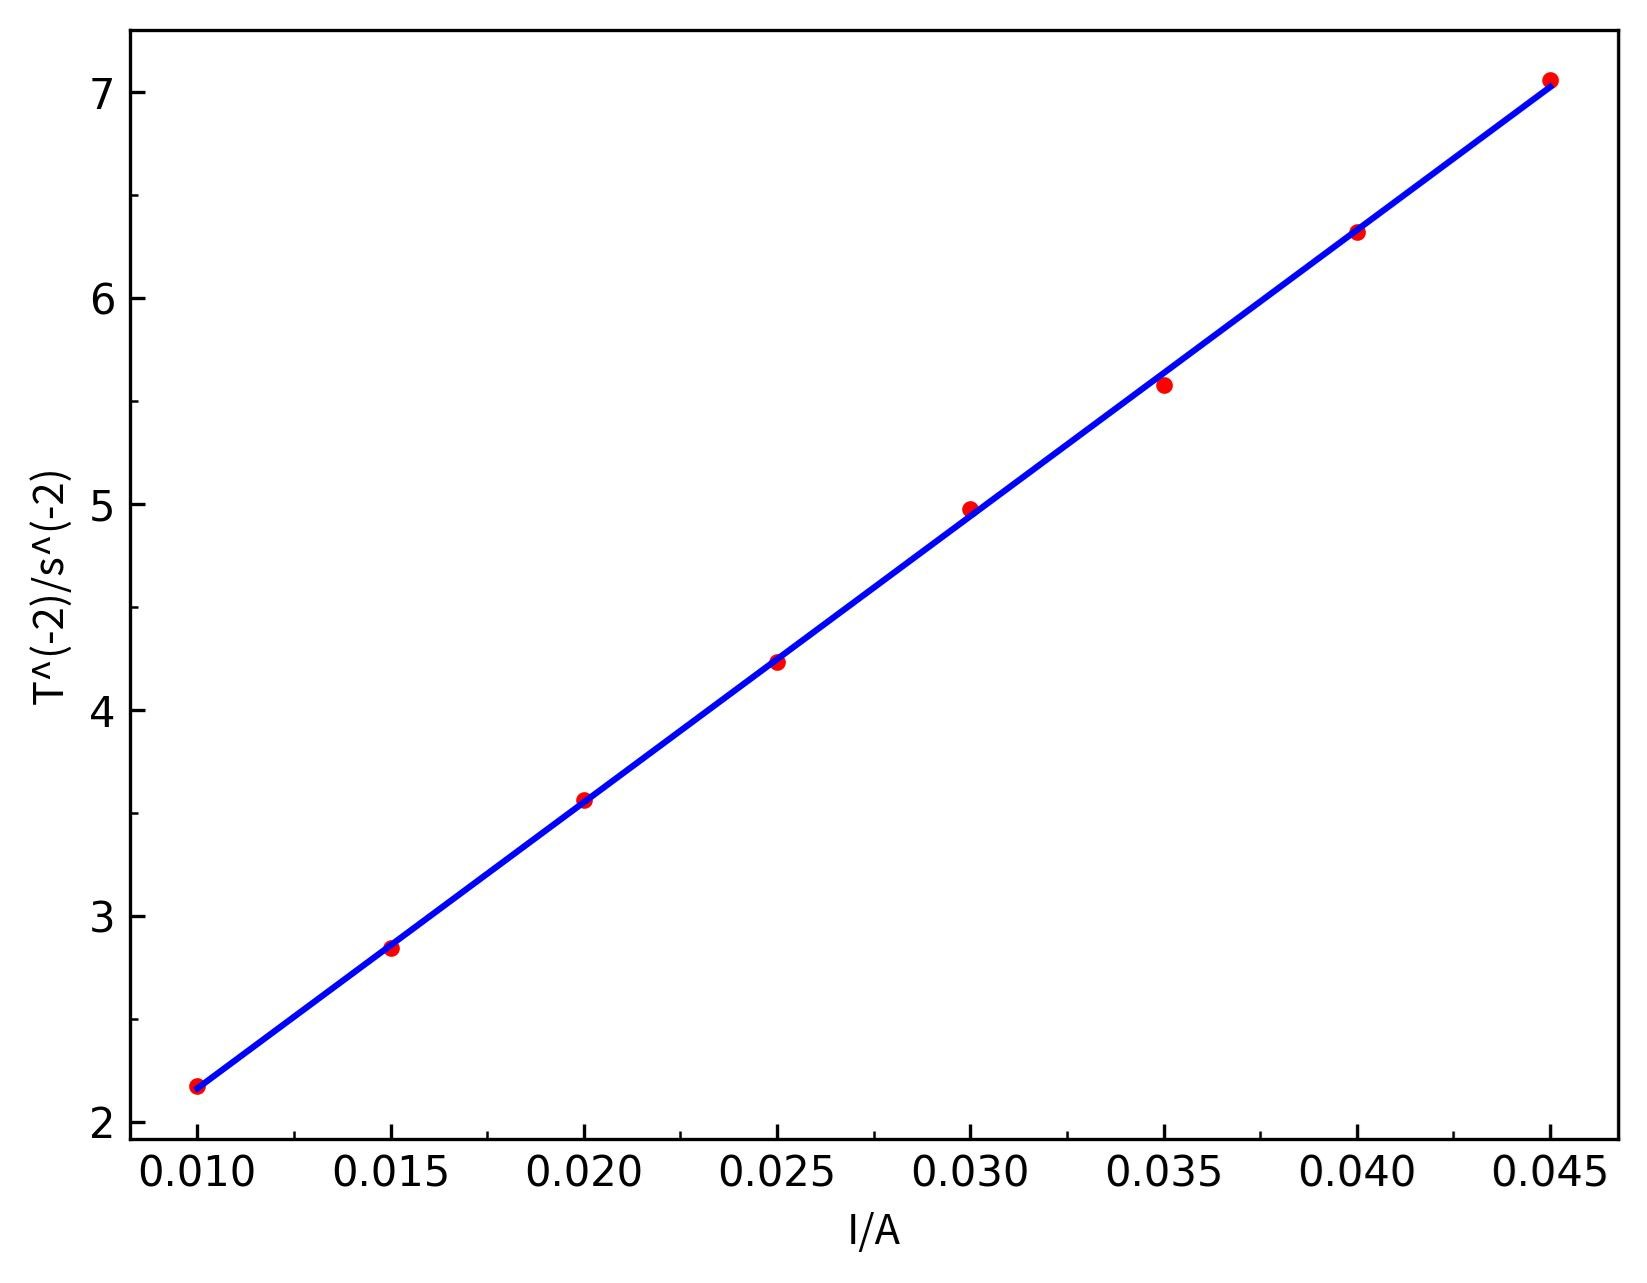
\includegraphics[width=0.8\textwidth]{周期与电流关系.jpg}
        \caption{\textbf{不同电流下磁力摆周期}}
    \end{figure}

    斜率
    \[
        a=138.96\,\mathrm{s^{-2}\cdot A^{-1}}
    \]
    截距
    \[
        b=0.77283\,\mathrm{s^{-2}}
    \]

    可知$a=\dfrac{m}{4\pi^2J}k$，$b=\dfrac{m}{4\pi^2J}B_0$，所以
    \[
        B_0=\frac{b}{a}k=\frac{0.77283}{138.96}\times 4.9524\approx0.02754\,\mathrm{mT}
    \]

\section{磁针磁矩和转动惯量}
    在地磁场中进行测量。

    小磁针长$2r=5.45\,\mathrm{cm}$，单个螺母质量$\mu=0.63\,\mathrm{g}$，不加螺母时周期$T_0=1.0969\,\mathrm{s}$，两边各加一个螺母时周期$T_1=1.4696\,\mathrm{s}$。
    
    由转动惯量定义，得
    \[
        J_1=J_0+2\mu r^2
    \]

    又由周期公式，得
    \[
        m=\frac{4\pi^2J_0}{T_0^2B_0}=\frac{4\pi^2J_1}{T_1^2B_0}
    \]
    从而可解得$m$和$J_0$：
    \[
        \left\{
        \begin{aligned}
            m&=\frac{8\pi^2\mu r^2}{B_0(T_1^2-T_0^2)} \\
            J_0&=\frac{2\mu r^2}{\frac{T_1^2}{T_0^2}-1}
        \end{aligned}
        \right.
    \]
    代入数据计算得
    \[
        m=1.4020\,\mathrm{A\cdot m^2},\quad J_0=1.1769\times 10^{-6}\,\mathrm{kg\cdot m^2}
    \]

\section{耦合运动}
    两个小磁针在地磁场中耦合运动，其耦合系数$k'$满足
    \[
        k'=\alpha\frac{m^2}{L^\beta}=\frac{1}{2}\left|\omega^2-{\omega^*}^2\right|
    \]
    其中，$\alpha$和$\beta$为常数，$L$为小磁针间距，$\omega$为同相运动时的角频率，$\omega^*$为反相运动时的角频率。

    对上式两边分别取对数，得
    \[
        \ln \alpha + 2\ln m - \beta \ln L = - \ln 2 + \ln\left|\omega^2-{\omega^*}^2\right|
    \]
    于是，可知$\ln\left|\omega^2-{\omega^*}^2\right|$与$\ln L$成线性关系。设$\ln\left|\omega^2-{\omega^*}^2\right|=u\ln L + v$，做出图象，并采用最小二乘法拟合得到（以下均采取国际单位制）：
    
    \begin{figure}[htbp]
        \centering
        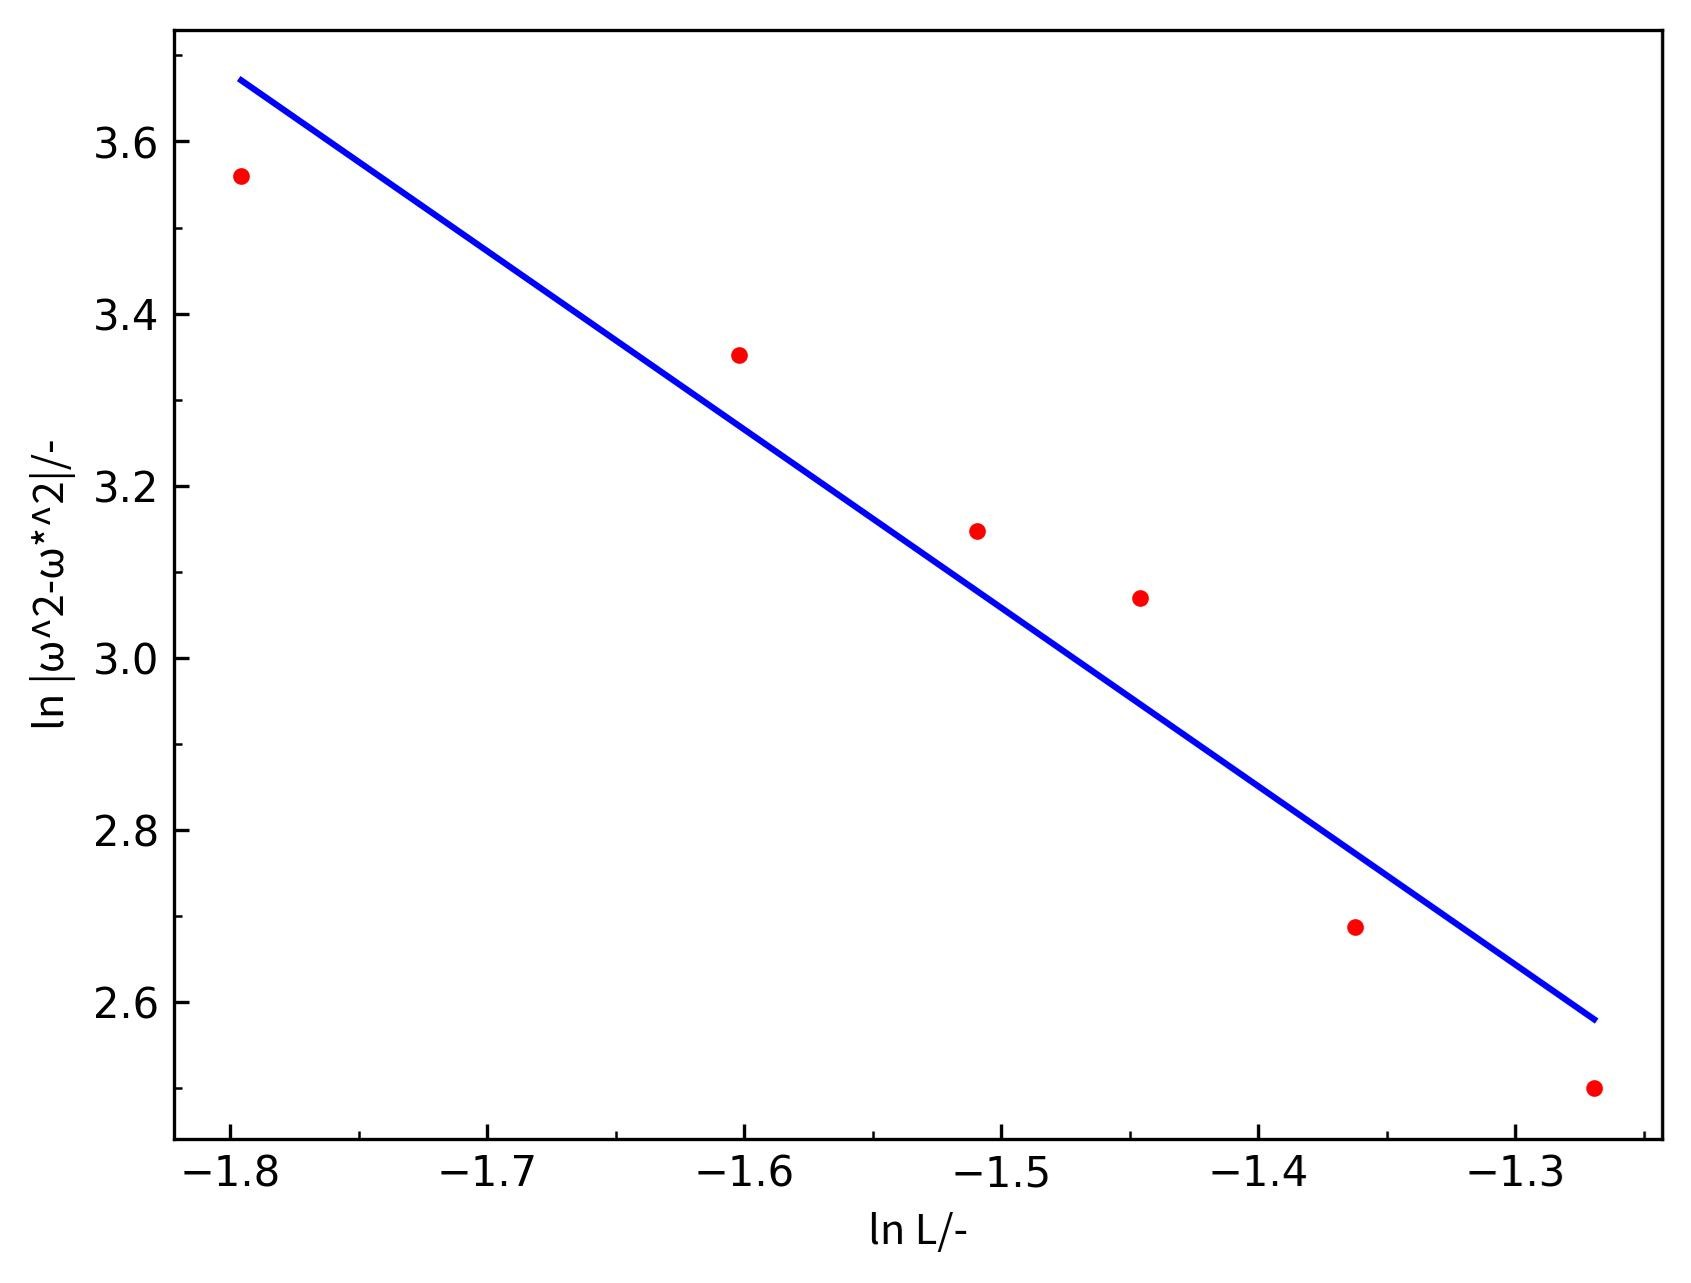
\includegraphics[width=0.8\textwidth]{耦合运动.jpg}
        \caption{\textbf{耦合运动}}
    \end{figure}

    斜率
    \[
        u=-2.0728
    \]
    截距
    \[
        v=-0.051172
    \]

    又
    \[
        u=-\beta,\quad v=\ln\alpha+2\ln m+\ln 2
    \]
    所以
    \[
        \alpha=\frac{e^v}{2m^2}\approx 0.2417,\quad \beta=-u\approx 2.0728
    \]

\appendix
\section{老师签字的原始数据}
    \begin{center}
        
\includegraphics[width=0.58\textwidth]{原始数据.jpg}
    \end{center}

\end{document}